\begin{figure}[H]%
		\ThisCenterWallPaper{1}{images/\texorpdfstring{\chaptername\thechapter}}%
		\captionlistentry[figure]{Icon of \chaptername\ \thechapter}% figure with chapter and section number
		%\addcontentsline{lof}{figure}{Icon of \chaptername\ \thechapter}% figure without chapter and section number
		\label{fig:\chaptername\thechapter}%
\end{figure}

\vspace*{-1.45cm}
\noindent \large{\textbf{This {\MakeLowercase{\chaptername}}'s contents:}}
\vspace*{-0.65cm}
\minitoc \mtcskip \minilof
\vspace*{-1.2cm}
\section{Project repositories} \label{section:SourceCode/Projectrepositories}
The work for this thesis is carried in different steps. Each phase and conceptually different workspace's source code is put in its own repository. All the repositories of the project are shown in \hyperref[longtable:repositories]{\autoref{longtable:repositories}}.

\begin{center}
	\vspace*{-0.25cm}
	\begin{longtable}{p{0.325\linewidth}p{0.62\linewidth}}
		\hline \hline
		\textbf{Description of the repo} & \textbf{URL to the repo} \\
		\hline \hline
		\endfirsthead
		
		\multicolumn{2}{l}{... continued from previous page}\\
		\hline \hline
		\textbf{Description of the repo} & \textbf{URL to the repo}\\
		\hline \hline
		\endhead
		
		\hline
		\caption*{\tablename\ \thetable{}: \nameref*{longtable:repositories}. Continues on next page ...}
		\vspace*{0.5cm}
		\endfoot
		
		\hline
		%\multicolumn{2}{| c |}{End of Table}\\
		%\hline
		\caption{All the repositories of the project.}\label{longtable:repositories}
		\vspace*{0.5cm}
		\endlastfoot

		XML to JSON conversion scripts & \url{github.com/A-Domain-that-Rocks/convert_large_xml_to_json} \\
		\hline
		Commands to import the JSON data in ArangoDB & \url{github.com/A-Domain-that-Rocks/arangodb_import_json_data} \\
		\hline
		\acrshort{AQL} Queries to edit collections, create nodes, edges and graphs from the imported data & \url{github.com/A-Domain-that-Rocks/distribute_data_in_arangodb} \\
		\hline
		Backend's source code & \url{github.com/A-Domain-that-Rocks/adomainthat-rocks_backend} \\
		\hline
		Frontend's source code & \url{github.com/A-Domain-that-Rocks/adomainthat-rocks_frontend} \\
		\hline
		Thesis's \LaTeX{} source code and PDF & \url{github.com/A-Domain-that-Rocks/masters_thesis} \\
		\hline
	\end{longtable}
	\vspace*{-1.35cm}
\end{center}

All the code is public, open and freely downloadable, or clonable/pullable with git.

\section{Instructions on how to run, build and deploy} \label{section:SourceCode/Instructionshowtorunbuildanddeploy}
\subsection{XML to JSON conversion scripts} \label{subsection:SourceCode/Instructionshowtorunbuildanddeploy/XMLtoJSONconversionscripts}
\noindent Open a terminal, change directory to where to store repo's source code and clone it:

\noindent\colorbox{lightestgray}{
	\parbox{1\linewidth-9pt}{%
		\texttt{\tiny\faDollarSign\large\ git clone https://github.com/A-Domain-that-Rocks/convert\_large\_xml\_to\_json.git}
	}%
}%

\medskip

\noindent Run the scripts with \gls{Python} or open and run them from an IDE.

\subsection{Commands to import the JSON data in ArangoDB} \label{subsection:SourceCode/Instructionshowtorunbuildanddeploy/CommandstoimporttheJSONdatainArangoDB}
\noindent Open a terminal, change directory to where to store repo's source code and clone it:

\noindent\colorbox{lightestgray}{
	\parbox{1\linewidth-9pt}{%
		\texttt{\tiny\faDollarSign\large\ git clone https://github.com/A-Domain-that-Rocks/arangodb\_import\_json\_data.git}
	}%
}%

\medskip

\noindent Run in bash the commands included in the files.

\subsection[AQL Queries to edit collections, create nodes, edges and graphs from the imported data]{\acrshort{AQL} Queries to edit collections, create nodes, edges and graphs from the imported data} \label{subsection:SourceCode/Instructionshowtorunbuildanddeploy/AQLQueriestoeditcollectionscreatenodesedgesandgraphsfromtheimporteddata}
\noindent Open a terminal, change directory to where to store repo's source code and clone it:

\noindent\colorbox{lightestgray}{
	\parbox{1\linewidth-9pt}{%
		\texttt{\tiny\faDollarSign\large\ git clone https://github.com/A-Domain-that-Rocks/distribute\_data\_in\_arangodb.git}
	}%
}%

\medskip

\noindent Copy commands in the ArangoDB web interface query editor and execute them.

\noindent For files \texttt{44\_de\-tec\-ting\_com\-mu\-ni\-ties.sh} and \texttt{45\_com\-mu\-ni\-ty\_de\-tec\-tion\_with\_pre\-gel.js}, execute those instructions in a terminal.

\subsection{Backend's source code} \label{subsection:SourceCode/Instructionshowtorunbuildanddeploy/Backendssourcecode}
\begin{figure}[H]%
	\centering%
	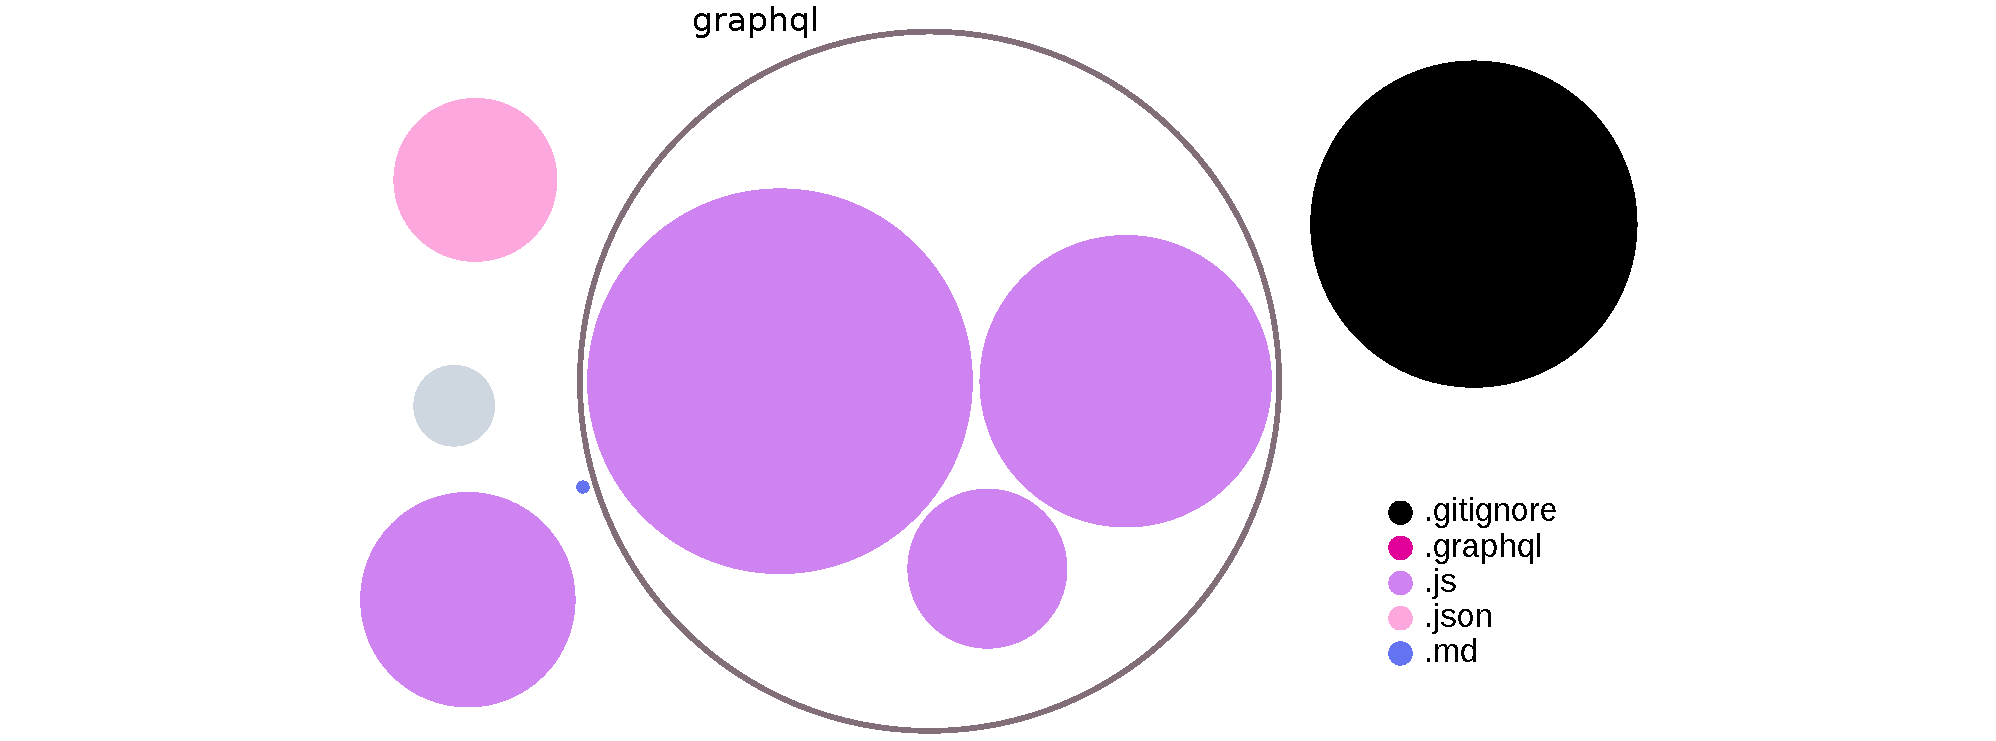
\includegraphics[width=1\textwidth]{images/appendixA/sourcecodebackendnew.pdf}%
	\caption[Backend's repo files]{Backend's repo files}%
	\label{fig:sourcecodebackendnew}%
\end{figure}%

\noindent Open a terminal, change directory to where to store repo's source code and clone it:

\noindent\colorbox{lightestgray}{
	\parbox{1\linewidth-9pt}{%
		\texttt{\tiny\faDollarSign\large\ git clone https://github.com/A-Domain-that-Rocks/adomainthat-rocks\_backend.git}
	}%
}%

\bigskip

\noindent \textbf{Run the app's backend/\acrshort{API} in localhost}:

\noindent Install NodeJS, instructions: \url{https://nodejs.org/en/download/}. NodeJS verion used 14.17.1 .

\noindent Change directory to inside the cloned repo:

\noindent\colorbox{lightestgray}{
	\parbox{1\linewidth-9pt}{%
		\texttt{\tiny\faDollarSign\large\ cd adomainthat-rocks\_backend}
	}%
}%

\medskip

\noindent Install all the project libraries:

\noindent\colorbox{lightestgray}{
	\parbox{1\linewidth-9pt}{%
		\texttt{\tiny\faDollarSign\large\ npm install}
	}%
}%

\medskip

\noindent Create a \texttt{.env} environment file to communicate with the database:

\noindent\colorbox{lightestgray}{
	\parbox{1\linewidth-9pt}{%
		\texttt{\tiny\faDollarSign\large\ echo -e "HOST=localhost \textbackslash nPORT=5000 \textbackslash n\textbackslash nDB\_HOST=localhost \textbackslash nDB\_NAME=db\_name \textbackslash nDB\_USER=root \textbackslash nDB\_PASS=pass \textbackslash n\textbackslash nAPI\_KEY=1234567890" >{}> .env}
	}%
}%

\medskip

\noindent Launch the app:

\noindent\colorbox{lightestgray}{
	\parbox{1\linewidth-9pt}{%
		\texttt{\tiny\faDollarSign\large\ npm start}
	}%
}%

\medskip

\noindent The \acrshort{API} endpoint is \url{http://localhost:5000/graphql}.
\bigskip

\noindent \textbf{Deploy the backend/\acrshort{API} on a web server.}

\noindent Copy the files to remote web server:

\noindent\colorbox{lightestgray}{
	\parbox{1\linewidth-9pt}{%
		\texttt{\tiny\faDollarSign\large\ ssh root@mydomain.com -p port "mkdir -p /root/api/" \&\& scp -P port -r /path/to/my/local/repositories/adomainthat-rocks\_backend/* root@mydomain.com:/root/api}
	}%
}%

\medskip

\noindent Install NodeJS on remote \acrshort{API} server machine, instructions: \url{https://nodejs.org/en/download/}. NodeJS version used: 14.17.1 .

\noindent Change directory to inside the cloned repo (run command on remote machine):

\noindent\colorbox{lightestgray}{
	\parbox{1\linewidth-9pt}{%
		\texttt{\tiny\faHashtag\large\ cd /root/api/}
	}%
}%

\medskip

\noindent Install all the project libraries (run command on remote machine):

\noindent\colorbox{lightestgray}{
	\parbox{1\linewidth-9pt}{%
		\texttt{\tiny\faHashtag\large\ npm install}
	}%
}%

\medskip

\noindent Create a \texttt{.env} environment file on remote \acrshort{API} server machine to communicate with the database host (run command on remote machine):

\noindent\colorbox{lightestgray}{
	\parbox{1\linewidth-9pt}{%
		\texttt{\tiny\faHashtag\large\ echo -e "HOST=databasehost.com \textbackslash nPORT=5000 \textbackslash n\textbackslash nDB\_HOST=databasehost.com \textbackslash nDB\_NAME=db\_name \textbackslash nDB\_USER=root \textbackslash nDB\_PASS=pass \textbackslash n\textbackslash nAPI\_KEY=1234567890" >{}> .env}
	}%
}%

\medskip

\noindent Install \texttt{PM2} Process Management daemon (run command on remote machine)

\noindent\colorbox{lightestgray}{
	\parbox{1\linewidth-9pt}{%
		\texttt{\tiny\faHashtag\large\ npm install -g pm2}
	}%
}%

\medskip

\noindent Start the \acrshort{API} server (run command on remote machine)

\noindent\colorbox{lightestgray}{
	\parbox{1\linewidth-9pt}{%
		\texttt{\tiny\faHashtag\large\ pm2 start /root/api/server.js}
	}%
}%

\noindent\colorbox{lightestgray}{
	\parbox{1\linewidth-9pt}{%
		\texttt{\tiny\faHashtag\large\ pm2 save}
	}%
}%

\medskip

\noindent The \acrshort{API} endpoint is \url{http://mydomain.com:5000/graphql}.

\subsection{Frontend's source code} \label{subsection:SourceCode/Instructionshowtorunbuildanddeploy/Frontendssourcecode}
\begin{figure}[H]%
	\centering%
	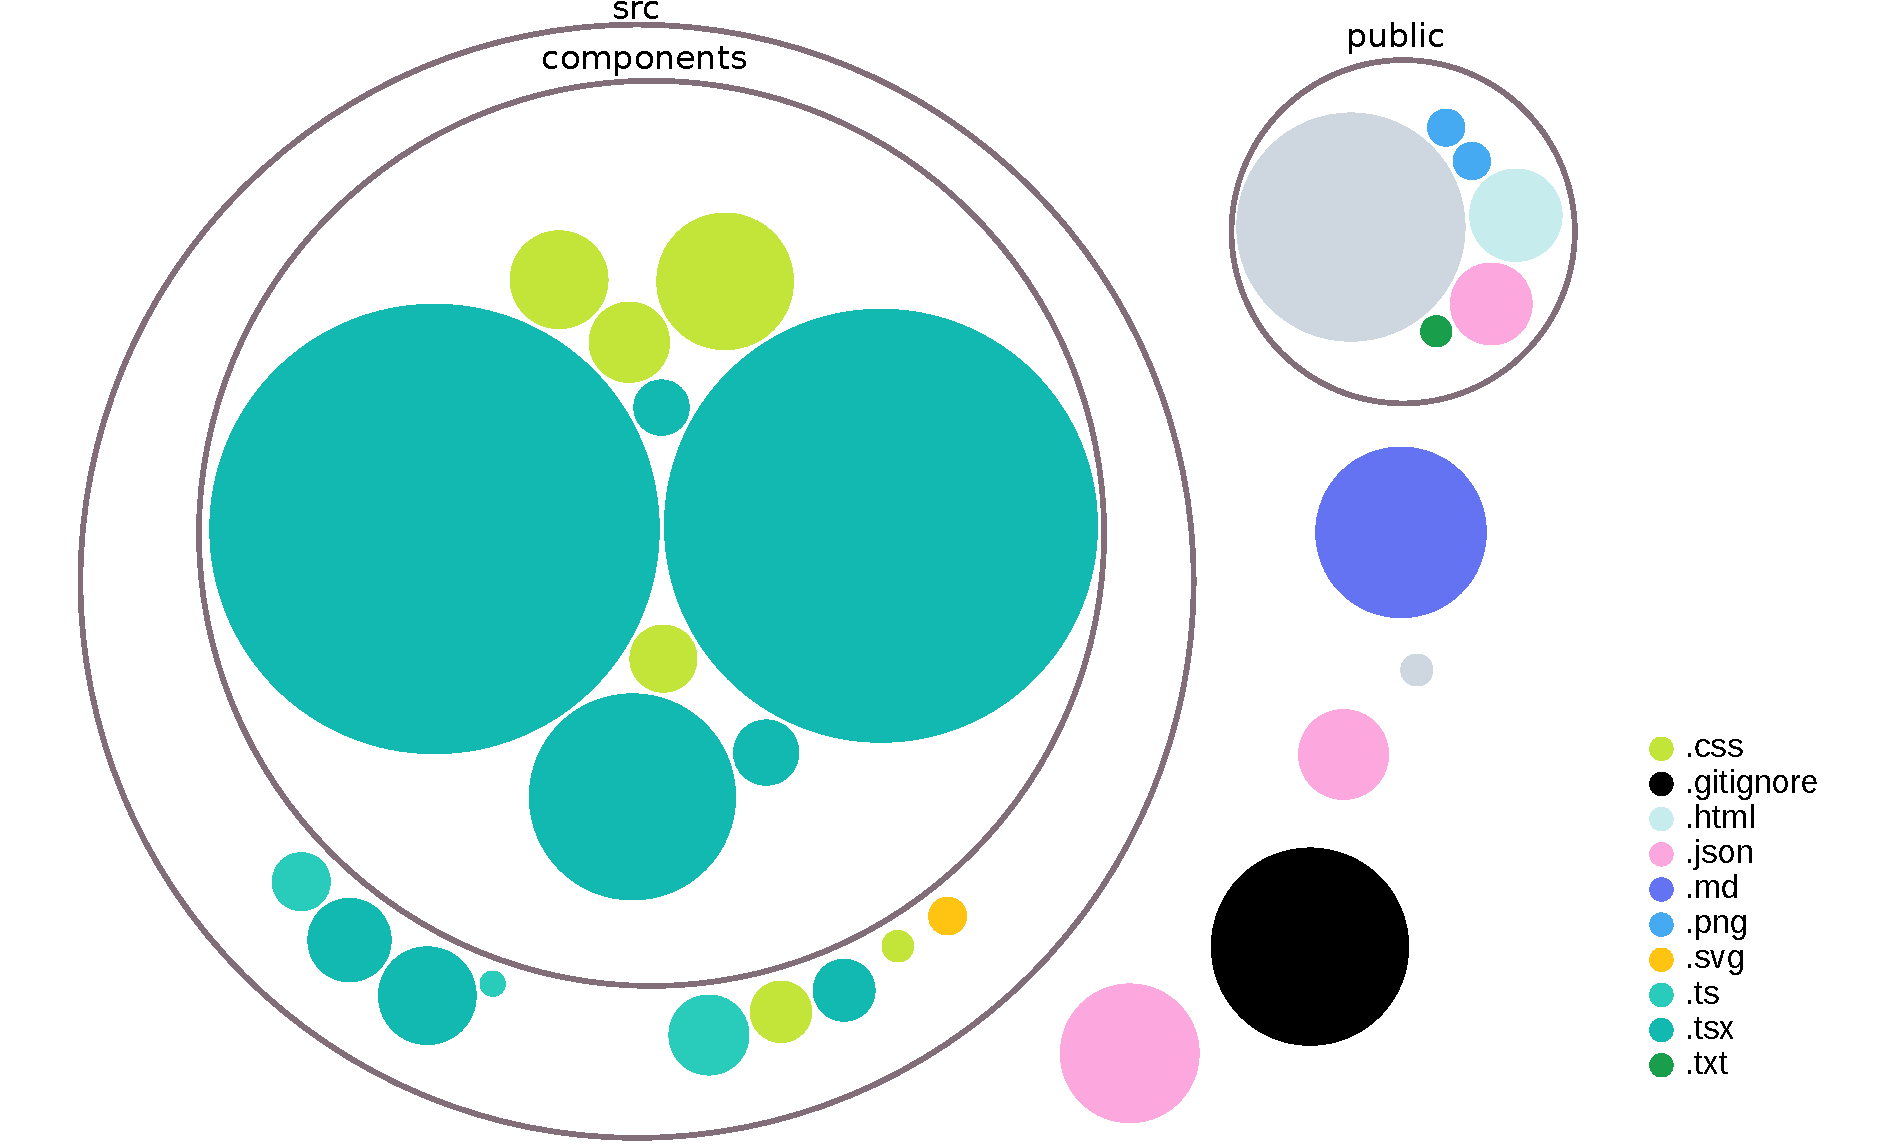
\includegraphics[width=1\textwidth]{images/appendixA/sourcecodefrontendnew.pdf}%
	\caption[Frontend's repo files]{Frontend's repo files}%
	\label{fig:sourcecodefrontendnew}%
\end{figure}%

\noindent Open a terminal, change directory to where to store repo's source code and clone it:

\noindent\colorbox{lightestgray}{
	\parbox{1\linewidth-9pt}{%
		\texttt{\tiny\faDollarSign\large\ git clone https://github.com/A-Domain-that-Rocks/adomainthat-rocks\_frontend.git}
	}%
}%

\medskip

\noindent Install NodeJS, instructions: \url{https://nodejs.org/en/download/}. NodeJS verion used 14.17.1 .

\noindent Change directory to inside the cloned repo:

\noindent\colorbox{lightestgray}{
	\parbox{1\linewidth-9pt}{%
		\texttt{\tiny\faDollarSign\large\ cd adomainthat-rocks\_frontend}
	}%
}%

\medskip

\noindent Install all the project libraries:

\noindent\colorbox{lightestgray}{
	\parbox{1\linewidth-9pt}{%
		\texttt{\tiny\faDollarSign\large\ npm install}
	}%
}%

\medskip

\noindent Create a \texttt{.env} environment file to communicate with the \acrshort{API}.

\noindent If the \acrshort{API} is in a remote machine: 

\noindent\colorbox{lightestgray}{
	\parbox{1\linewidth-9pt}{%
		\texttt{\tiny\faDollarSign\large\ echo 'REACT\_APP\_API\_URL=http://mydomain.com:5000/graphql' >{}> .env}
	}%
}%

\medskip

\noindent If the \acrshort{API} is in localhost:

\noindent\colorbox{lightestgray}{
	\parbox{1\linewidth-9pt}{%
		\texttt{\tiny\faDollarSign\large\ echo 'REACT\_APP\_API\_URL=http://localhost:5000/graphql' >{}> .env}
	}%
}%
\bigskip

\noindent \textbf{Run the app's client interface in localhost}:

\noindent Launch the app:

\noindent\colorbox{lightestgray}{
	\parbox{1\linewidth-9pt}{%
		\texttt{\tiny\faDollarSign\large\ npm start}
	}%
}%

\medskip

\noindent If the app did not automatically open in the browser, visit \url{http://localhost:3000/}.
\bigskip

\noindent \textbf{Build the Web App interface and deploy on a web server.}

\noindent Build the app:

\noindent\colorbox{lightestgray}{
	\parbox{1\linewidth-9pt}{%
		\texttt{\tiny\faDollarSign\large\ npm run build}
	}%
}%

\medskip

\noindent Copy the built app to remote web server:

\noindent\colorbox{lightestgray}{
	\parbox{1\linewidth-9pt}{%
		\texttt{\tiny\faDollarSign\large\ scp -P port -r /path/to/my/local/repositories/adomainthat-rocks\_frontend/build/* root@mydomain.com:/var/www/html/}
	}%
}%

\medskip

\noindent Open firewall ports (run commands on remote machine):

\noindent\colorbox{lightestgray}{
	\parbox{1\linewidth-9pt}{%
		\texttt{\tiny\faHashtag\large\ firewall-cmd -{}-permanent -{}-zone=public -{}-add-service=http}
	}%
}%

\noindent\colorbox{lightestgray}{
	\parbox{1\linewidth-9pt}{%
		\texttt{\tiny\faHashtag\large\ firewall-cmd -{}-permanent -{}-zone=public -{}-add-service=https}
	}%
}%

\noindent\colorbox{lightestgray}{
	\parbox{1\linewidth-9pt}{%
		\texttt{\tiny\faHashtag\large\ firewall-cmd -{}-reload}
	}%
}%

\medskip

\noindent Enable Apache to start automatically on boot (run commands on remote machine):

\noindent\colorbox{lightestgray}{
	\parbox{1\linewidth-9pt}{%
		\texttt{\tiny\faHashtag\large\ systemctl enable httpd}
	}%
}%

\noindent\colorbox{lightestgray}{
	\parbox{1\linewidth-9pt}{%
		\texttt{\tiny\faHashtag\large\ systemctl restart httpd.service}
	}%
}%

\noindent\colorbox{lightestgray}{
	\parbox{1\linewidth-9pt}{%
		\texttt{\tiny\faHashtag\large\ apachectl restart}
	}%
}%

\medskip

\noindent Visit \url{http://mydomain.com}.

\subsection{Thesis's \LaTeX{} source code} \label{subsection:SourceCode/Instructionshowtorunbuildanddeploy/ThesissLatexsourcecode}
\begin{figure}[H]%
	\centering%
	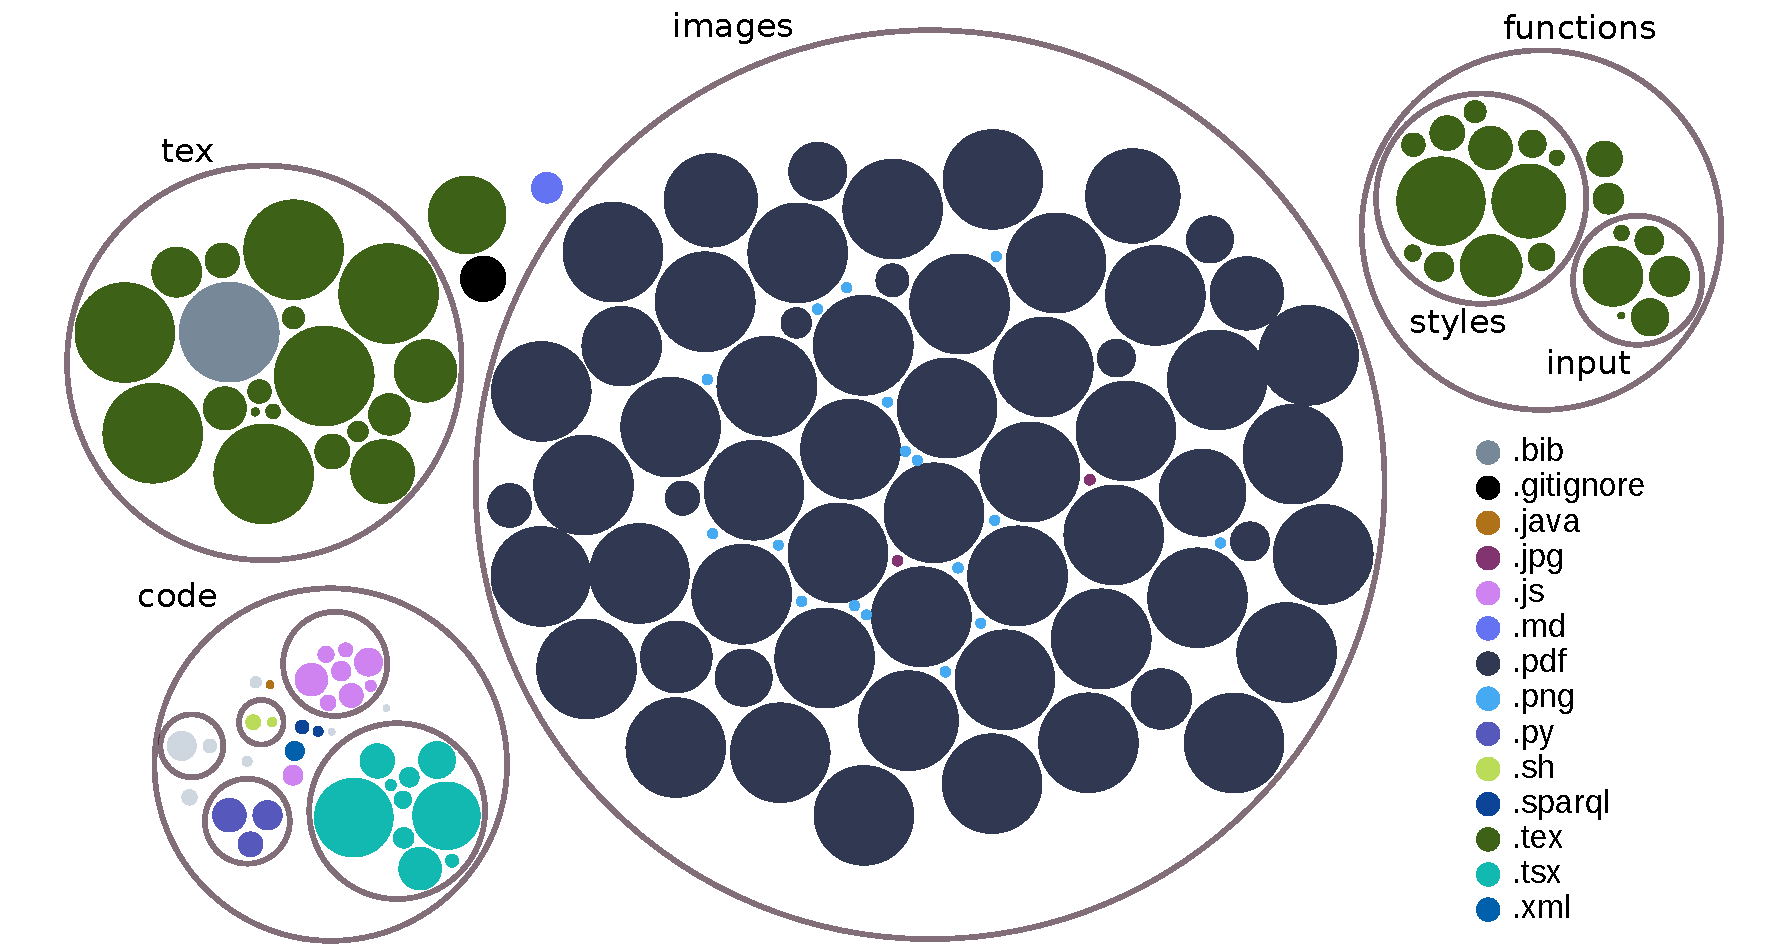
\includegraphics[width=1\textwidth]{images/appendixA/sourcecodethesisnew.pdf}%
	\caption[Thesis's repo files]{Thesis's repo files}%
	\label{fig:sourcecodethesisnew}%
\end{figure}%

\noindent \textbf{Compile with Overleaf}

\noindent Open a terminal, change directory to where to store repo's ZIP archive and download it:

\noindent\colorbox{lightestgray}{
	\parbox{1\linewidth-9pt}{%
		\texttt{\tiny\faDollarSign\large\ curl -L https://github.com/A-Domain-that-Rocks/masters\_thesis/archive/refs/heads/main.zip -{}-out\-put mas\-ters\_the\-sis\_\myauthorname\_\myauthorsurname.zip}
	}%
}%

\medskip

\noindent Open \url{https://www.overleaf.com/project} \adforn{43} \colorbox{darkgreen}{\parbox{3cm}{\centering \textcolor{white}{New Project}}} \adforn{43} Upload Project \adforn{43} \textit{Upload the previously down\-load\-ed} \texttt{mas\-ters\_the\-sis\_\myauthorname\_\myauthorsurname.zip} \textit{file} \adforn{43} \colorbox{darkgreen}{\parbox{3cm}{\centering \textcolor{white}{\faSync*\ Recompile}}}
\bigskip

\noindent \textbf{Compile locally}

\noindent Install a \TeX{} or \LaTeX{} \glspl{compiler}. Clone the repo:

\noindent\colorbox{lightestgray}{
	\parbox{1\linewidth-9pt}{%
		\texttt{\tiny\faDollarSign\large\ git clone https://github.com/A-Domain-that-Rocks/masters\_thesis.git}
	}%
}%

\medskip

\noindent Install the packages used in the project. Compile the project locally.

\newpage
\thispagestyle{empty}
